% 2010 年山东卷文科第 20 题：多面体 P-ABCD 与点 M、E、G、F。
% 来源 PDF：普通高考/2010/2010山东文.pdf，SHA-256 95a69b861a29ca594f9118c9643efcdfd04cae3c4f374ff9fa009f7ac99712f4。
% 原页：第 2 页（A3 三栏）第 1 栏下部，书页码 622。
% 重绘依据：ABCD 为正方形；MA⊥平面 ABCD，PD∥MA，AD=PD=2MA；
%   E、G、F 分别为 MB、PB、PC 的中点；P-D 与 A-D 为不可见棱，画虚线。
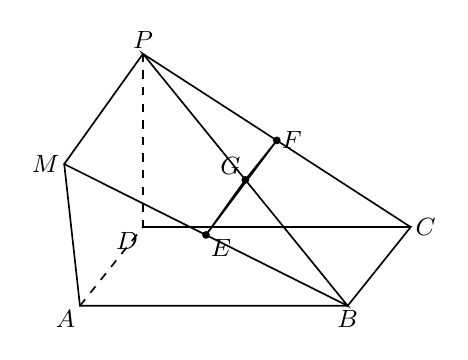
\begin{tikzpicture}[semithick, every node/.style={inner sep=1.5pt, font=\small}]
  \coordinate (A) at (0,0);
  \coordinate (B) at (3.4,0);
  \coordinate (C) at (4.2,1.0);
  \coordinate (D) at (0.8,1.0);
  \coordinate (M) at (-0.2,1.8);
  \coordinate (P) at (0.8,3.2);
  \coordinate (E) at (1.6,0.9);
  \coordinate (F) at (2.5,2.1);
  \coordinate (G) at (2.1,1.6);

  \draw (M) -- (A) -- (B) -- (C) -- (D);
  \draw (P) -- (M) -- (B) -- (P) -- (C);
  \draw[dashed] (P) -- (D);
  \draw[dashed] (A) -- (D);
  \draw (E) -- (F) -- (G) -- cycle;

  \fill (E) circle (1.4pt);
  \fill (F) circle (1.4pt);
  \fill (G) circle (1.4pt);
  \node[left] at (M) {$M$};
  \node[above] at (P) {$P$};
  \node[below left] at (A) {$A$};
  \node[below] at (B) {$B$};
  \node[right] at (C) {$C$};
  \node[below left] at (D) {$D$};
  \node[below right] at (E) {$E$};
  \node[right] at (F) {$F$};
  \node[above left] at (G) {$G$};
\end{tikzpicture}
